\documentclass[letterpaper, 10pt]{article}
\usepackage[margin=2cm]{geometry}

\usepackage{amssymb}
\usepackage{graphicx}
\usepackage{subfig}

\setlength{\parindent}{0em}
\setlength{\parskip}{0.3em}

\title{\textbf{18-748 Wireless Sensor Networks Lab 2}}
\author{Emily Ruppel, Iljoo Baek, Mengwen He}

\begin{document}
	\maketitle
	
We deployed a centralized architecture for this Whack-a-Mole project following the skeleton code; therefore, our development focused on the master node whose framework is shown as Fig.\ref{fig:framework}.

\begin{figure}[!h]
	\centering
	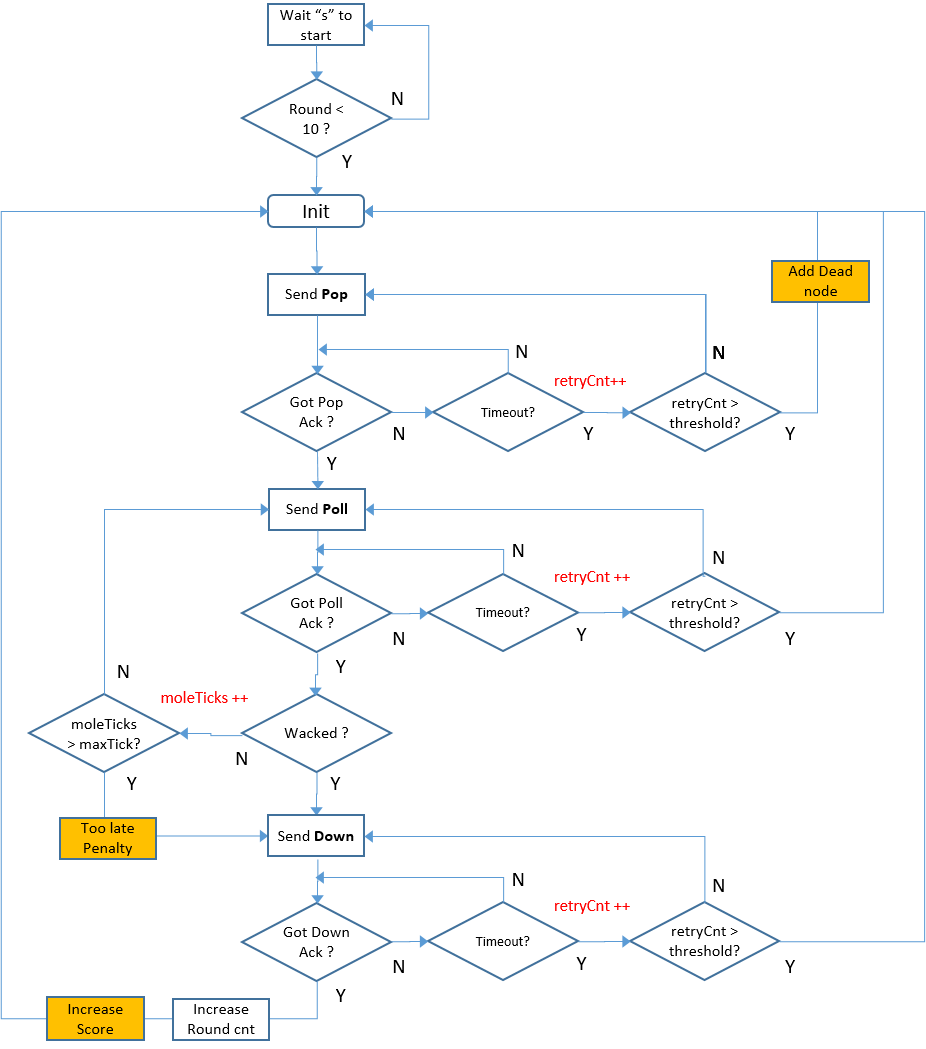
\includegraphics[width=13cm]{./frame.png}
	\caption{Framework of the master node.}
	\label{fig:framework}
\end{figure}

The slave nodes are controlled by the master node via the Pop-Poll-Down order sequence for each round. In the Pop stage, the master will find all the valid slaves and randomly wake up one. In the Poll stage, the master will continuously query the status of target slave node to catch the whack event. In the Down stage, the score will be changed according to the response of target slave node.

\begin{itemize}
	\item The system-latency in terms of the worst case time for a mole to wake up: As shown in the framework, the response time of waking up a mole is the time cost of the Pop stage; therefore, the worst case of a successful pop stage equals to ``retryCnt-threshold" $\times$ ``the time interval to wait for the Pop Ack".
	\item The life-time of slave nodes powered by batteries: for each round, the slaves node need to work in Pop and Poll stages. In the Pop stage, all active slave nodes need to reply the acknowledgment of pop query, assuming $a$ J consumed. In the Poll stage, only on active slave node need to continuously reply the light measurement of each poll query, assuming $b$ J / poll query; therefore, the total energy consumed is $b\times$ maxTick. Assume there are N slave nodes and the choosing of a slave follows the uniform distribution, then the estimated energy consumption of a slave node is $(a+b\times$maxTick$)/N$ for each round, and thus the estimated life-time of a slave node is $E\times N/(a+b\times$maxTick$)$, where $E$ is the total energy of two AA batteries.
\end{itemize}

\end{document}